\documentclass[handout,instructornotes]{ximera}
%handout:  for handout version with no solutions or instructor notes
%handout,instructornotes:  for instructor version with just problems and notes, no solutions
%noinstructornotes:  shows only problem and solutions

%% handout
%% space
%% newpage
%% numbers
%% nooutcomes

%I added the commands here so that I would't have to keep looking them up
%\newcommand{\RR}{\mathbb R}
%\renewcommand{\d}{\,d}
%\newcommand{\dd}[2][]{\frac{d #1}{d #2}}
%\renewcommand{\l}{\ell}
%\newcommand{\ddx}{\frac{d}{dx}}
%\everymath{\displaystyle}
%\newcommand{\dfn}{\textbf}
%\newcommand{\eval}[1]{\bigg[ #1 \bigg]}

%\begin{image}
%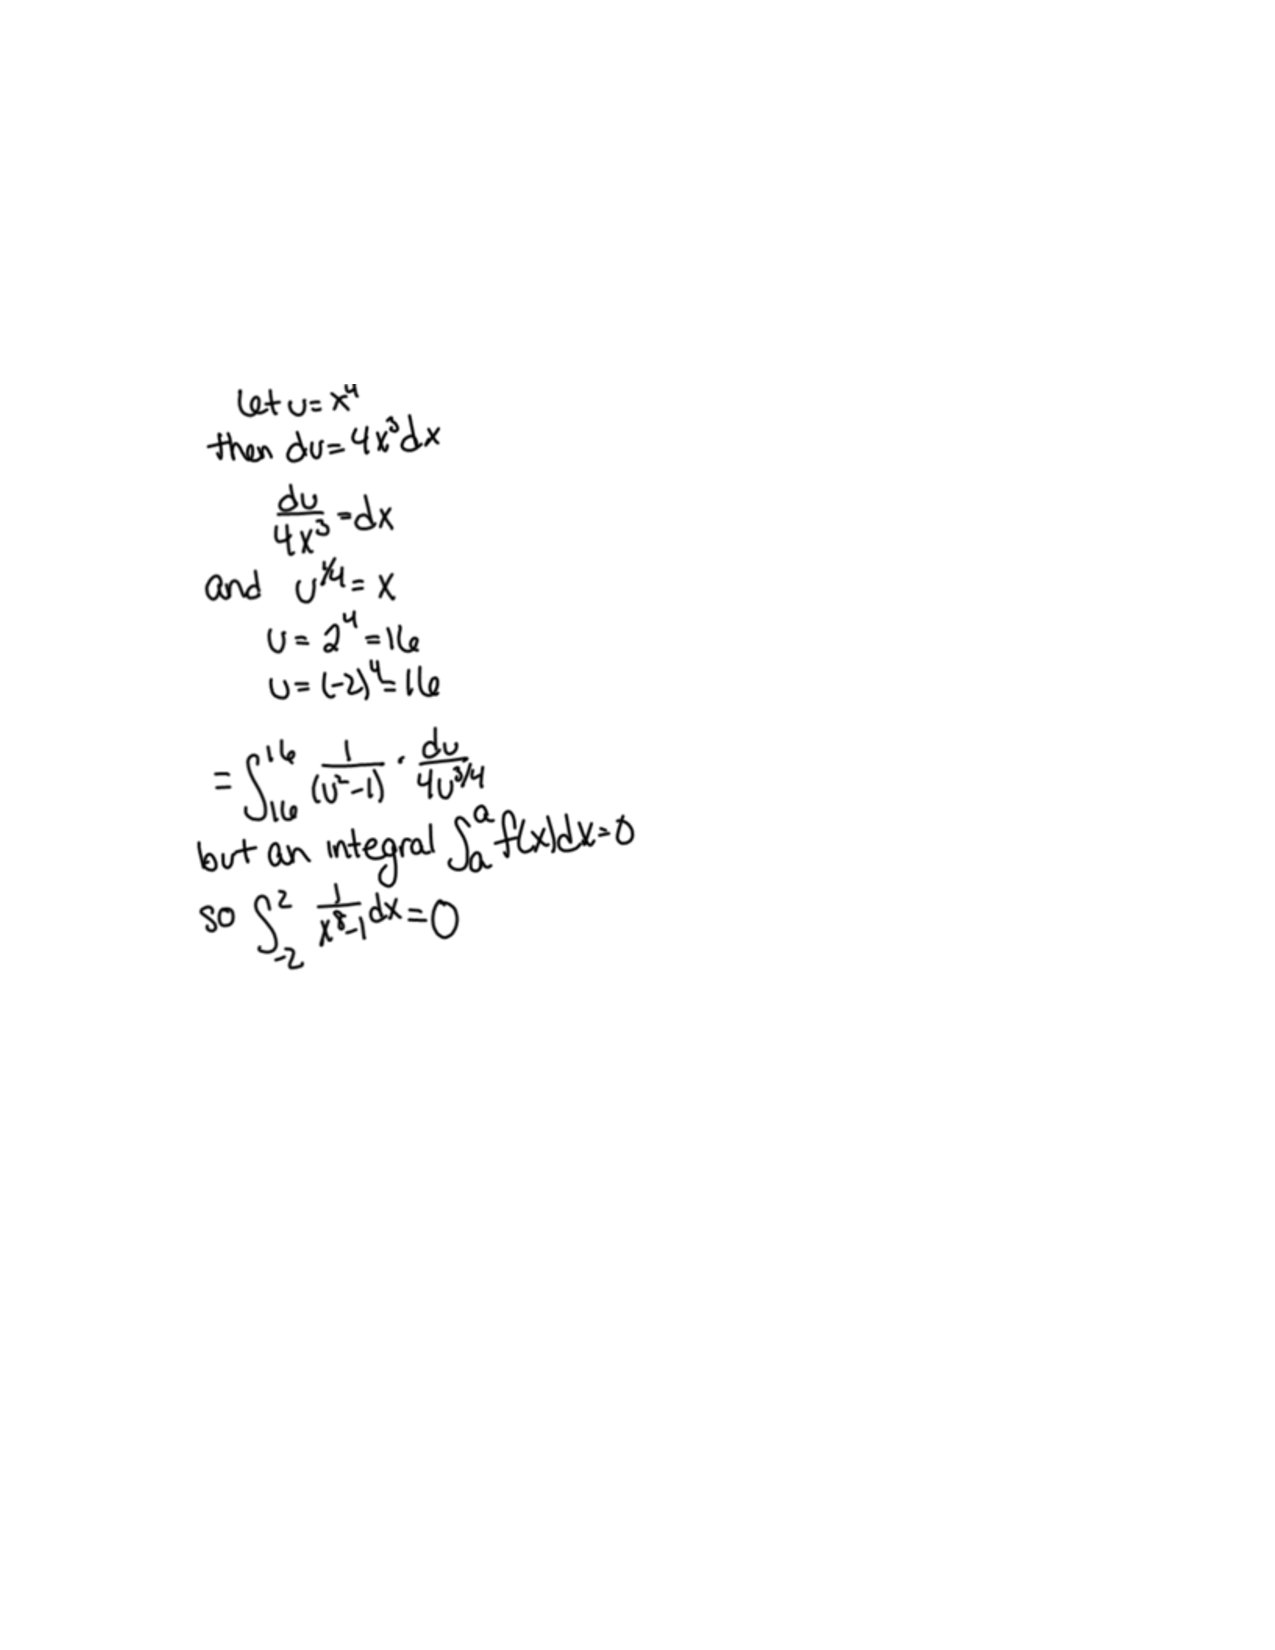
\includegraphics[trim= 170 420 250 180]{Figure1.pdf}
%\end{image}

%add a ``.'' below when used in a specific directory.
\newcommand{\RR}{\mathbb R}
\renewcommand{\d}{\,d}
\newcommand{\dd}[2][]{\frac{d #1}{d #2}}
\renewcommand{\l}{\ell}
\newcommand{\ddx}{\frac{d}{dx}}
\newcommand{\dfn}{\textbf}
\newcommand{\eval}[1]{\bigg[ #1 \bigg]}

\usepackage{multicol}

\renewenvironment{freeResponse}{
\ifhandout\setbox0\vbox\bgroup\else
\begin{trivlist}\item[\hskip \labelsep\bfseries Solution:\hspace{2ex}]
\fi}
{\ifhandout\egroup\else
\end{trivlist}
\fi} %% we can turn off input when making a master document

\title{Recitation \# 3: Volume by Slicing \& Shells}  

\begin{document}
\begin{abstract}		\end{abstract}
\maketitle



%again, no real warm-up for this section.
\begin{comment}
\section{Warm up:}

	\begin{freeResponse}
	
	\end{freeResponse}
	
\begin{instructorNotes}

\end{instructorNotes}
\end{comment}







\section{Group work:}



%problem 1
\begin{problem}
	\begin{enumerate}
		\item  Consider the region bounded by the curves $y=x^2+8$ and $y=7x-2$.  
		Set up an integral that will compute the volume of the solid whose base is the region and whose cross sections perpendicular to the region and the $x$-axis are:
			\begin{enumerate}
				\item[(i)]  Equilateral triangles
				\begin{freeResponse}
				We first set the curves equal to each other to see where they intersect
					\begin{align*}
					x^2 + 8 &= 7x - 2  \\
					x^2 - 7x + 10 &= 0  \\
					(x-2)(x-5) &= 0  \\
					x &= 2,5.
					\end{align*}
				By checking the point $x=3$, we see that $7x-2 \geq x^2+8$ over the interval $[2,5]$.  
				So our region is bounded
					\begin{itemize}
					\item  from above by $y=7x-2$
					\item  from below by $y=x^2+8$
					\item  from the left by  $x=2$
					\item  from the right by $x=5$.
					\end{itemize}
					
				Now, recall that an equilateral triangle is a triangle where the length of each side is the same.  
				If we let $s$ denote the common side length of an equilateral triangle, then we can use Pythagorean's Theorem to solve for the height $h$:
				\[
				h^2 + \left( \frac{1}{2} s \right)^2 = s^2 \qquad \Longrightarrow \qquad h = \frac{\sqrt{3}}{2} s.
				\]
				Then the area $A$ of this equilateral triangle is
				\[
				A = \frac{1}{2} \cdot s \cdot h = \frac{\sqrt{3}}{4} s^2.
				\]
				
				The volume of the solid that we are trying to find is given by the integral
				\[
				\int_2^5 A(x) \d x
				\]
				where $A(x)$ is the area of an equilateral triangle (within in the region and perpendicular to the $x$-axis) at a generic point $x$.  
				The base of such a triangle is given by $s(x) = (7x-2) - (x^2+8) = -x^2 + 7x -10$ (see the picture below).  
				Thus,
				\[
				A(x) = \frac{\sqrt{3}}{4} s(x)^2 = \frac{\sqrt{3}}{4} (-x^2+7x-10)^2
				\]
				and
				\[
				\text{{\color{red} Volume of region}} = \int_2^5 \frac{\sqrt{3}}{4} (-x^2+7x-10)^2 \d x .
				\]
				
					\begin{image}
					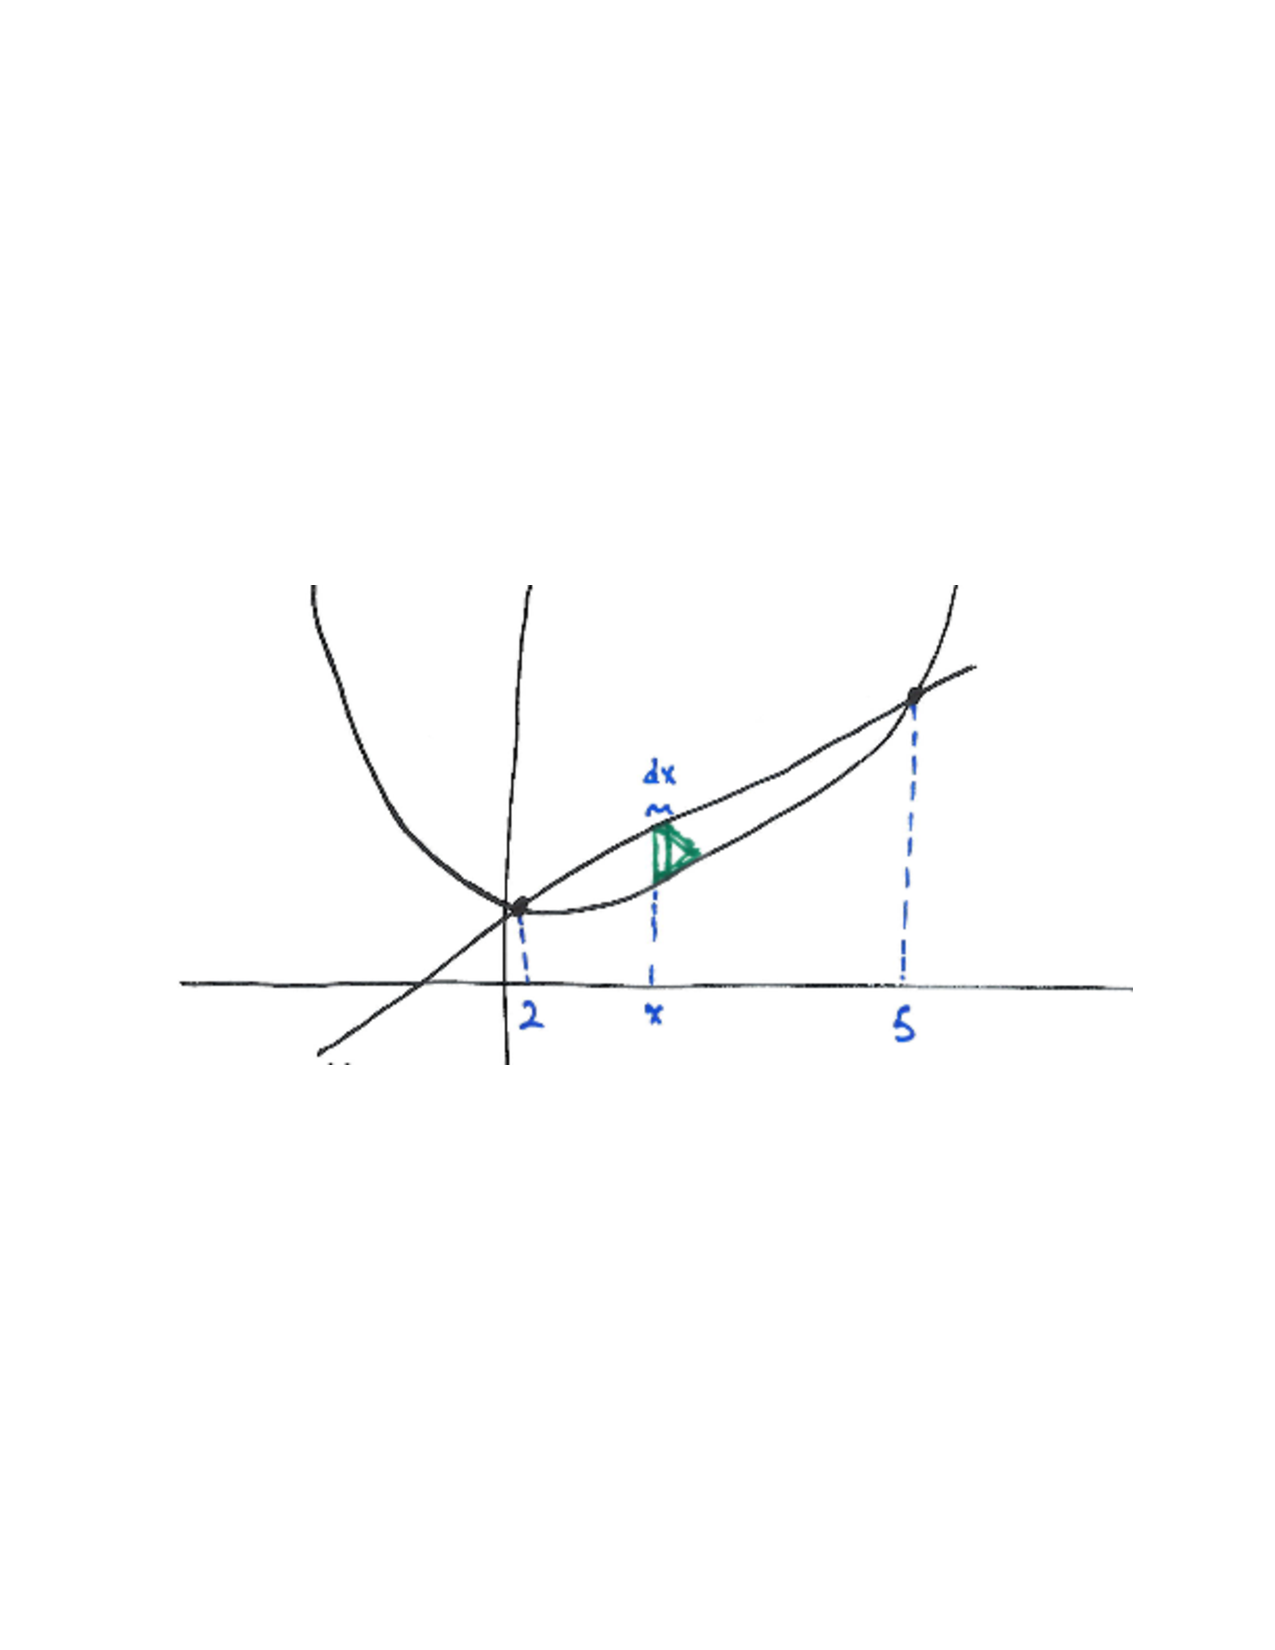
\includegraphics[trim= 240 280 200 270, scale=0.8]{Figure6-3-2.pdf}
					\end{image}
				\end{freeResponse}
				
				\item[(ii)]  Semicircles
				\begin{freeResponse}
				Everything is exactly the same as in part (a), except now each slice is a semicircle instead of an equilateral triangle.  
				Recall that the area of half of a circle is $\frac{\pi}{2} r^2$, and at a generic point $x$ the radius satisfies
				\[  
				2r(x) = -x^2+7x-10	\qquad	\Longrightarrow		\qquad	r^2(x) = \frac{1}{4} \left( -x^2+7x-10 \right)^2.
				\]
				Then we have that
					\begin{align*}
					\text{{\color{red} Volume of region}} &= \int_2^5 A(x) \d x  \\
					&= \int_2^5 \frac{\pi}{2} \cdot \frac{1}{4} \left( -x^2+7x-10 \right)^2 \d x  \\
					&= \frac{\pi}{8} \int_2^5 \left( -x^2+7x-10 \right)^2 \d x.
					\end{align*}
				\end{freeResponse}
			\end{enumerate}
		
		\item  Do the same as in (a), except that the solid's cross-sections are perpendicular to the region and the $y$-axis.
		\begin{freeResponse}
			\begin{enumerate}
			\item[(i)] Equilateral triangles.
			
			The structure of this problem is the same as in part (a).  
			We know that the two curves intersect at $x=2,5$, and so plugging those into either equation shows that the $y$-coordinates of these intersection points are $y=12, 33$.  
			Over the region $12 \leq y \leq 33$ we can solve both equations for $x$
				\begin{align*}
				x_1 &= \sqrt{y-8}  \\
				x_2 &= \frac{1}{7} (y+2).
				\end{align*}
			By either checking a point in the interval $[12,33]$ or simply by consulting the picture above, we see that $x_1 \geq x_2$ over this region.  
			Then the base of an equilateral triangle at a generic point $y$ is
				\[
				s(y) = \sqrt{y-8} - \frac{1}{7}(y+2)
				\]
			and the volume of the region is
				\begin{align*}
				\text{{\color{red} Volume of region}} &= \int_{12}^{33} A(y) \d y  \\
				&= \int_{12}^{33} \frac{\sqrt{3}}{4} \left( \sqrt{y-8} - \frac{1}{7}(y+2) \right)^2 \d y.
				\end{align*}
			
			\item[(ii)] Semicircles
			Again, we proceed in exactly the same way as in part (a).  
			From above, we have that
				\[  
				2r(y) = \sqrt{y-8} - \frac{1}{7}(y+2)	\qquad	\Longrightarrow		\qquad	r^2(y) = \frac{1}{4} \left( \sqrt{y-8} - \frac{1}{7}(y+2) \right)^2
				\]
			and
				\begin{align*}
				\text{{\color{red} Volume of region}} &= \int_{12}^{33} A(y) \d y  \\
				&= \int_{12}^{33} \frac{\pi}{2} \cdot \frac{1}{4} \left( \sqrt{y-8} - \frac{1}{7}(y+2) \right)^2 \d y  \\
				&= \frac{\pi}{8} \int_{12}^{33} \left( \sqrt{y-8} - \frac{1}{7}(y+2) \right)^2 \d y.
				\end{align*}
			
			\end{enumerate}
		\end{freeResponse}
	\end{enumerate}
	
\end{problem}

\begin{instructorNotes}
Do 1(a)(i) as a class.  
Have the students do 1(a)(ii) in groups and have a group present.  
Then split the two parts of (b) between the groups.  
Discuss as a class. 
\end{instructorNotes}







%problem 2
\begin{problem}
Set up an integral that will find the volume of the solid formed by revolving the region bounded by the curves $y=x^2-4x+8$ and $y=-x^2+10x-12$ about:

\begin{image}
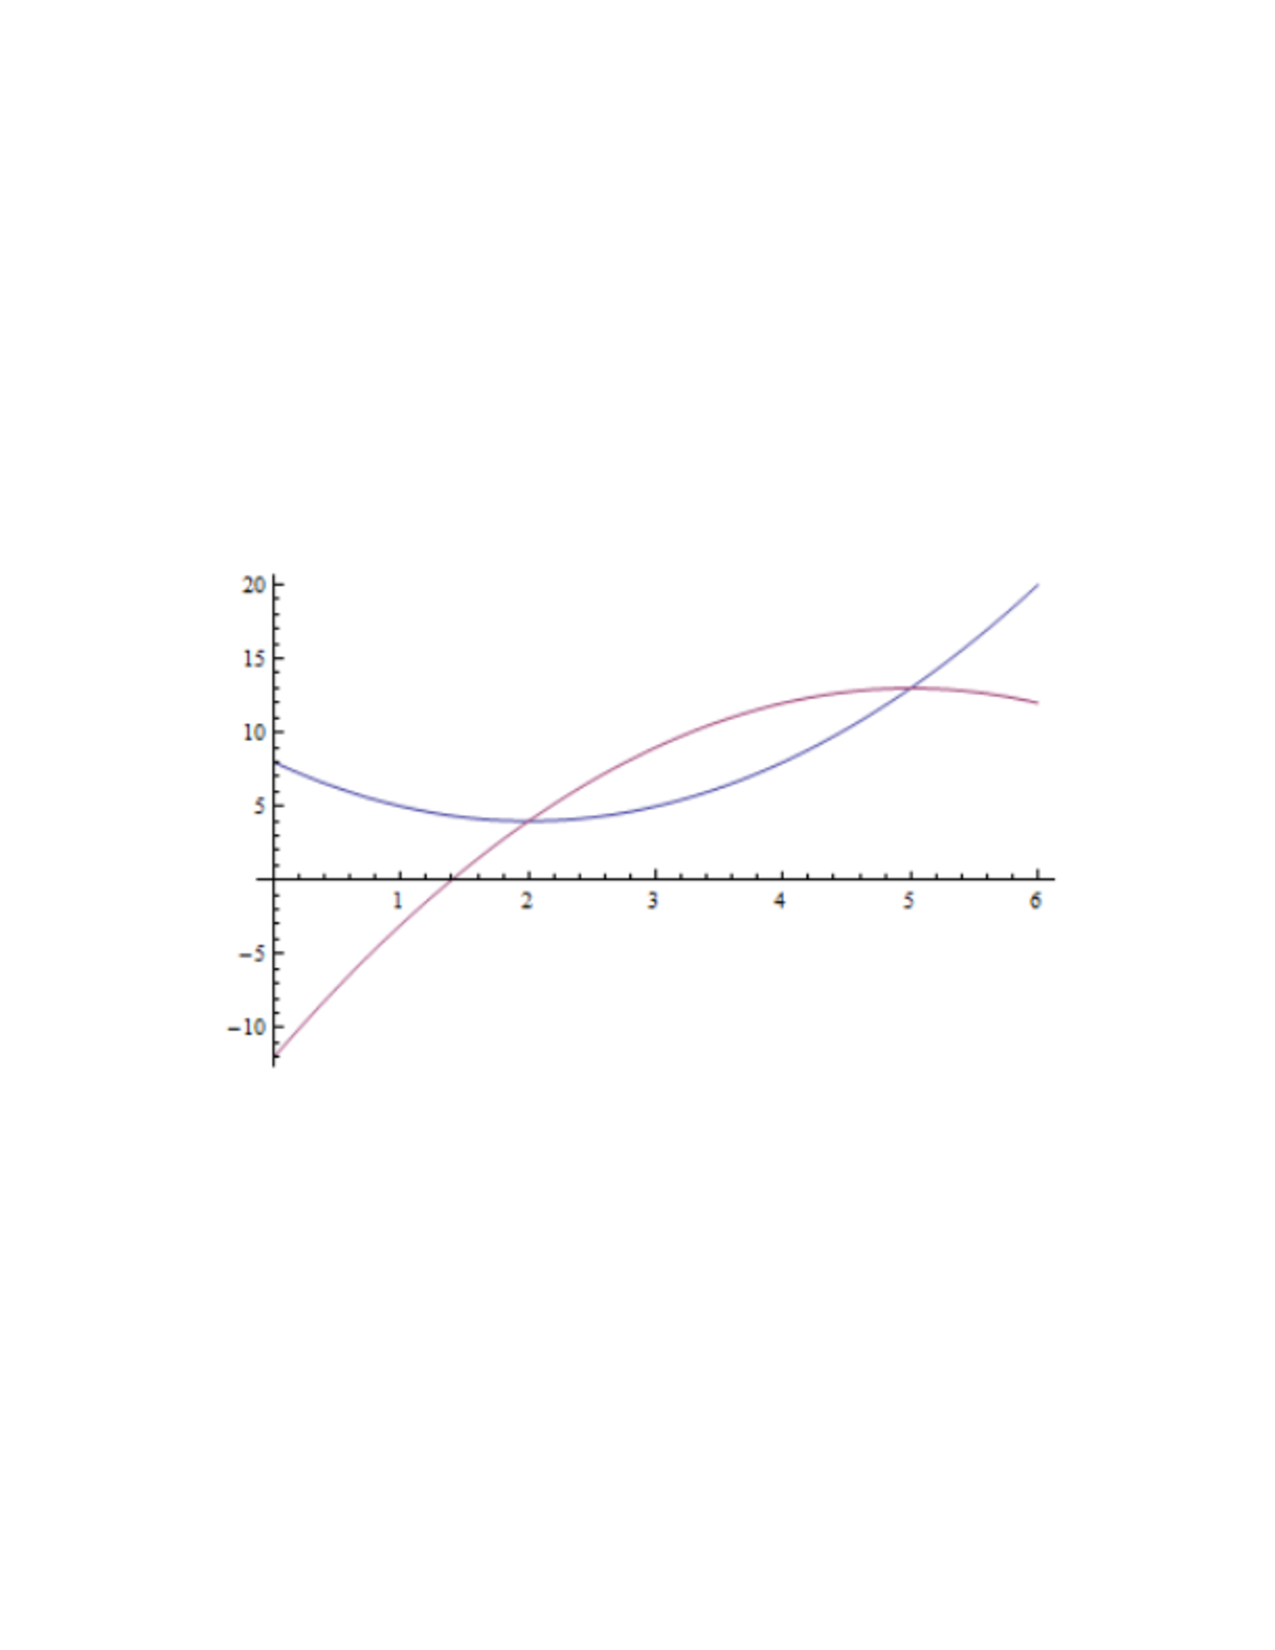
\includegraphics[trim= 240 280 200 270, scale=0.8]{Figure6-3-1.pdf}
\end{image}
	
	\begin{enumerate}
		\item  the $x$-axis
		\begin{freeResponse}
		First, we need to find where the two curves intersect
			\begin{align*}
			x^2-4x+8 &= -x^2+10x-12  \\
			2x^2 -14x +20 &= 0  \\
			x^2 - 7x + 10 &= 0  \\
			(x-2)(x-5) &= 0  \\
			x &= 2,5.
			\end{align*}
		By plugging in the point $x=3$, we see that
			\[
			-x^2+10x-12 \geq x^2-4x+8
			\]
		on the interval $[2,5]$.  
		
		Notice that a cross section at a generic point $x$ looks like a ``washer".  
		Thus, to find the volume of the surface of revolution, we need to compute
			\[
			\int_2^5 A(x) \d x
			\]
		where $A(x)$ denotes the area of the corresponding washer.  
		Recall that $A(x) = \pi \left( r_{out}^2 - r_{in}^2 \right)$ where $r_{out}$ and $r_{in}$ denote the outside and inside radius of the washer, respectively.  
		Consulting the picture, we see that
			\begin{align*}
			r_{out} &= -x^2+10x-12  \\
			r_{in} &= x^2-4x+8
			\end{align*}
		and thus
			\[
			\text{{\color{red} Volume of region}} = \pi \int_2^5 \left[ (-x^2+10x-12)^2 - (x^2-4x+8)^2 \right] \d x.
			\]
			
		\begin{image}
		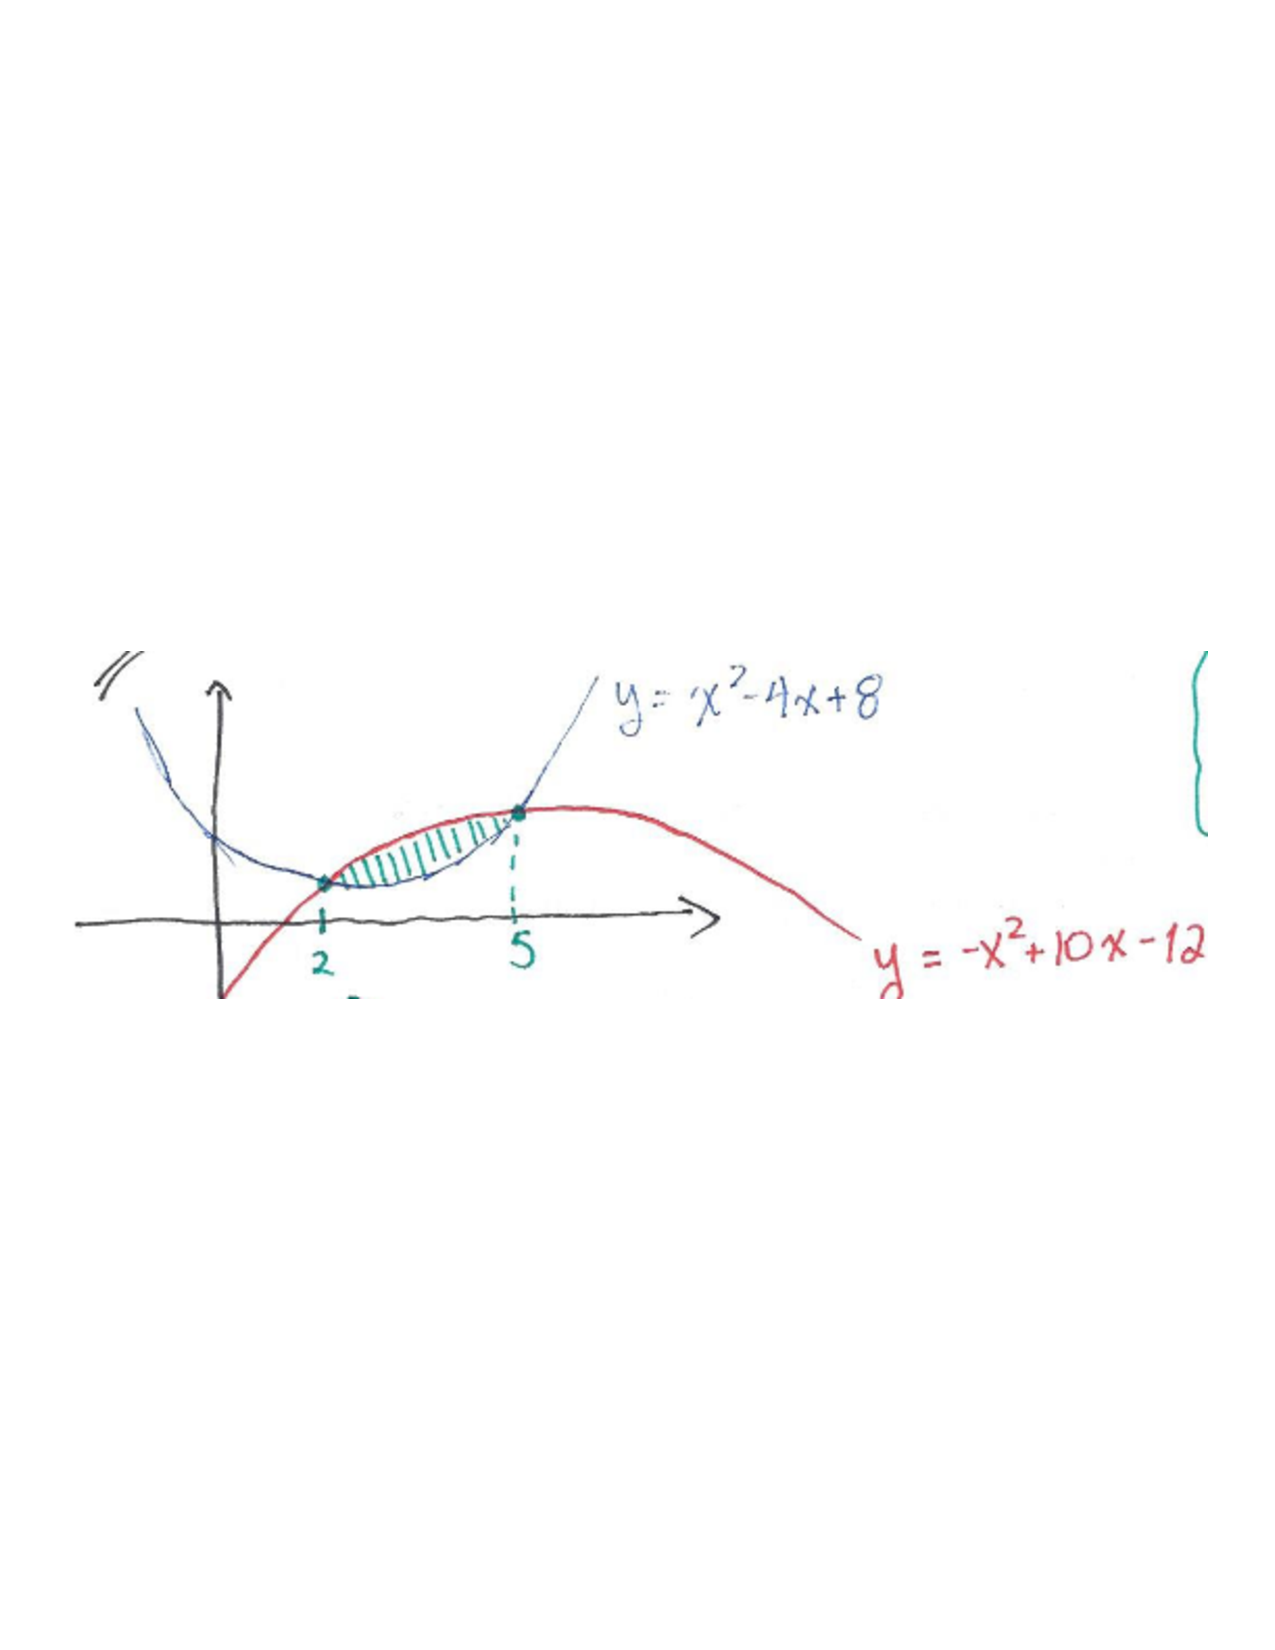
\includegraphics[trim= 240 290 200 310, scale=0.8]{Figure6-3-3.pdf}
		\end{image}
		
		\begin{image}
		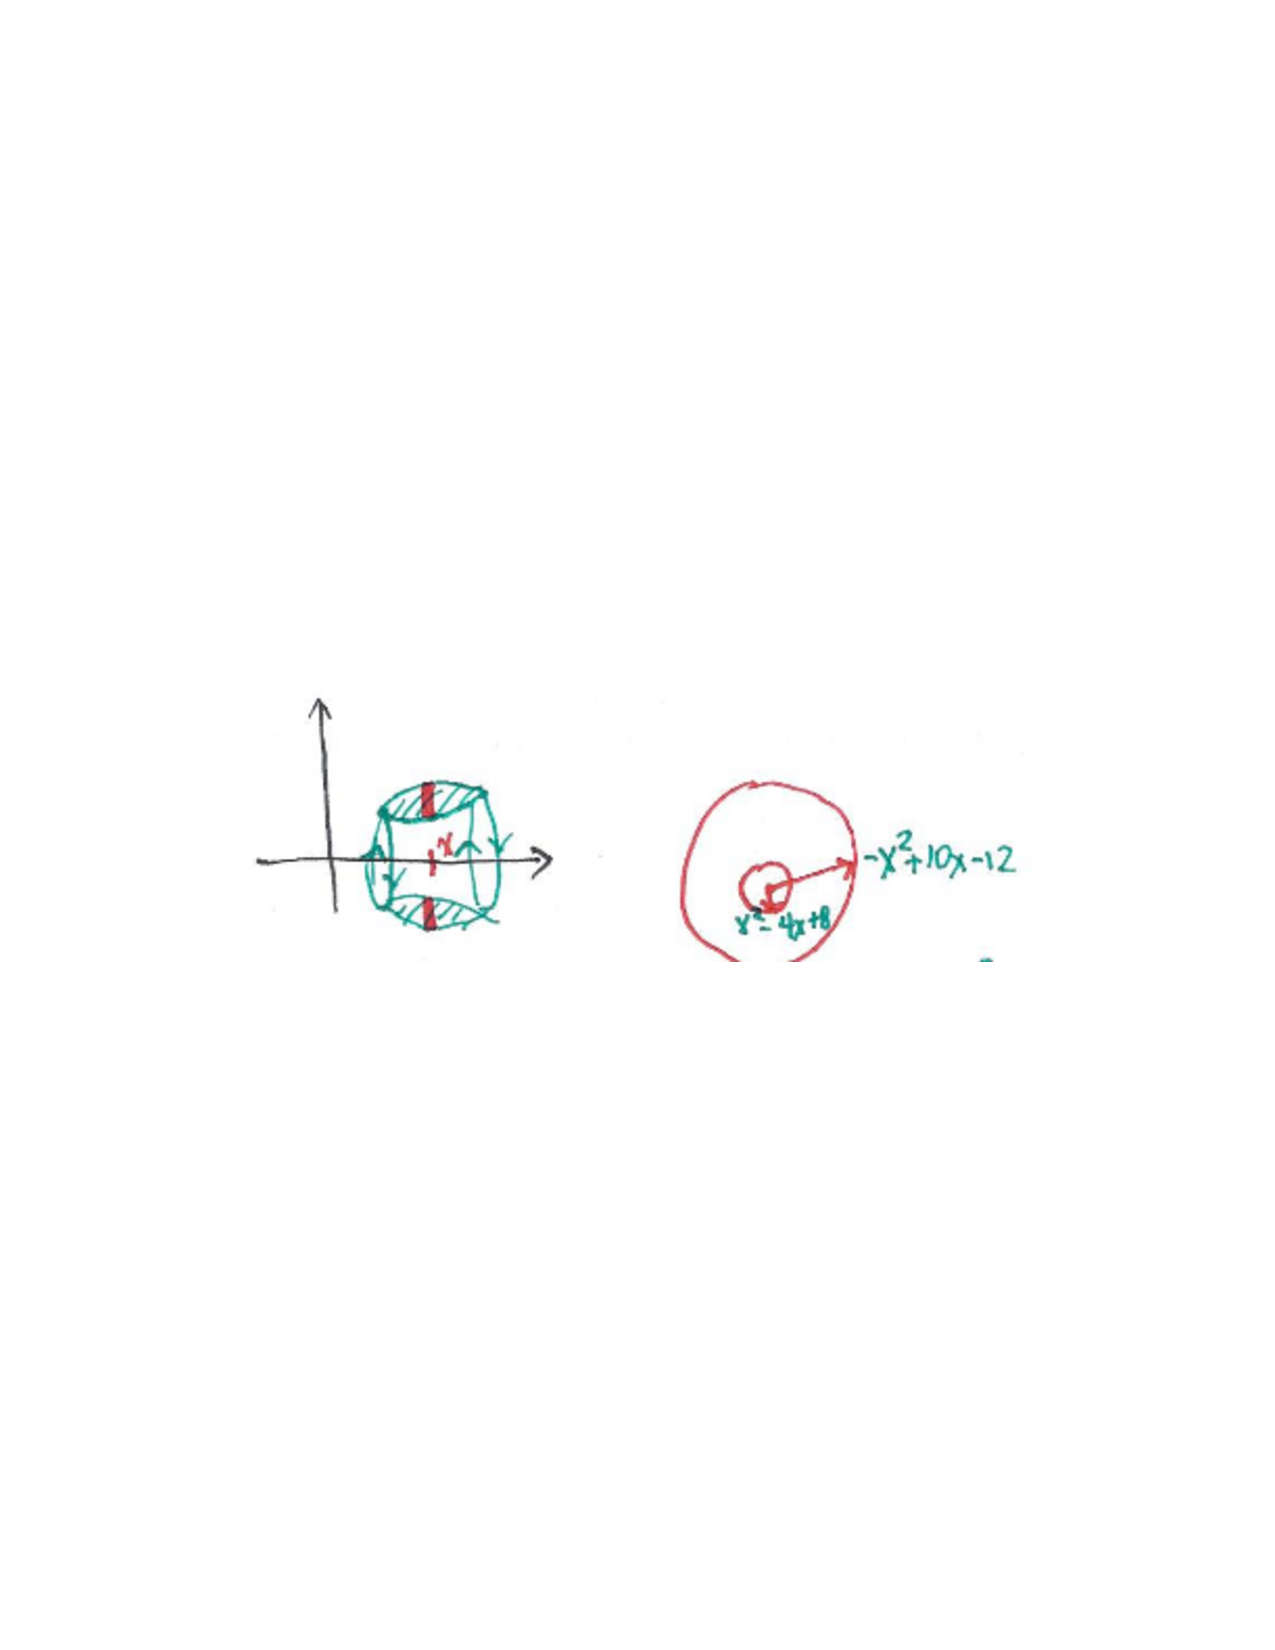
\includegraphics[trim= 240 320 200 330, scale=0.8]{Figure6-3-4.pdf}
		\end{image}
		\end{freeResponse}
		
		
		
		\item  $y=-3$
		\begin{freeResponse}
		The line $y=-3$ is just the $x$-axis shifted down $3$ units.  
		So both radii just ``grow" by $3$:
			\begin{align*}
			r_{out} &= 3 + (-x^2+10x-12) = -x^2 + 10x -9  \\
			r_{in} &= 3 + (x^2-4x+8) = x^2 - 4x + 11.
			\end{align*}
		Then
			\[
			\text{{\color{red} Volume of region}} = \pi \int_2^5 \left[ (-x^2+10x-9)^2 - (x^2-4x+11)^2 \right] \d x.
			\]
			
		\begin{image}
		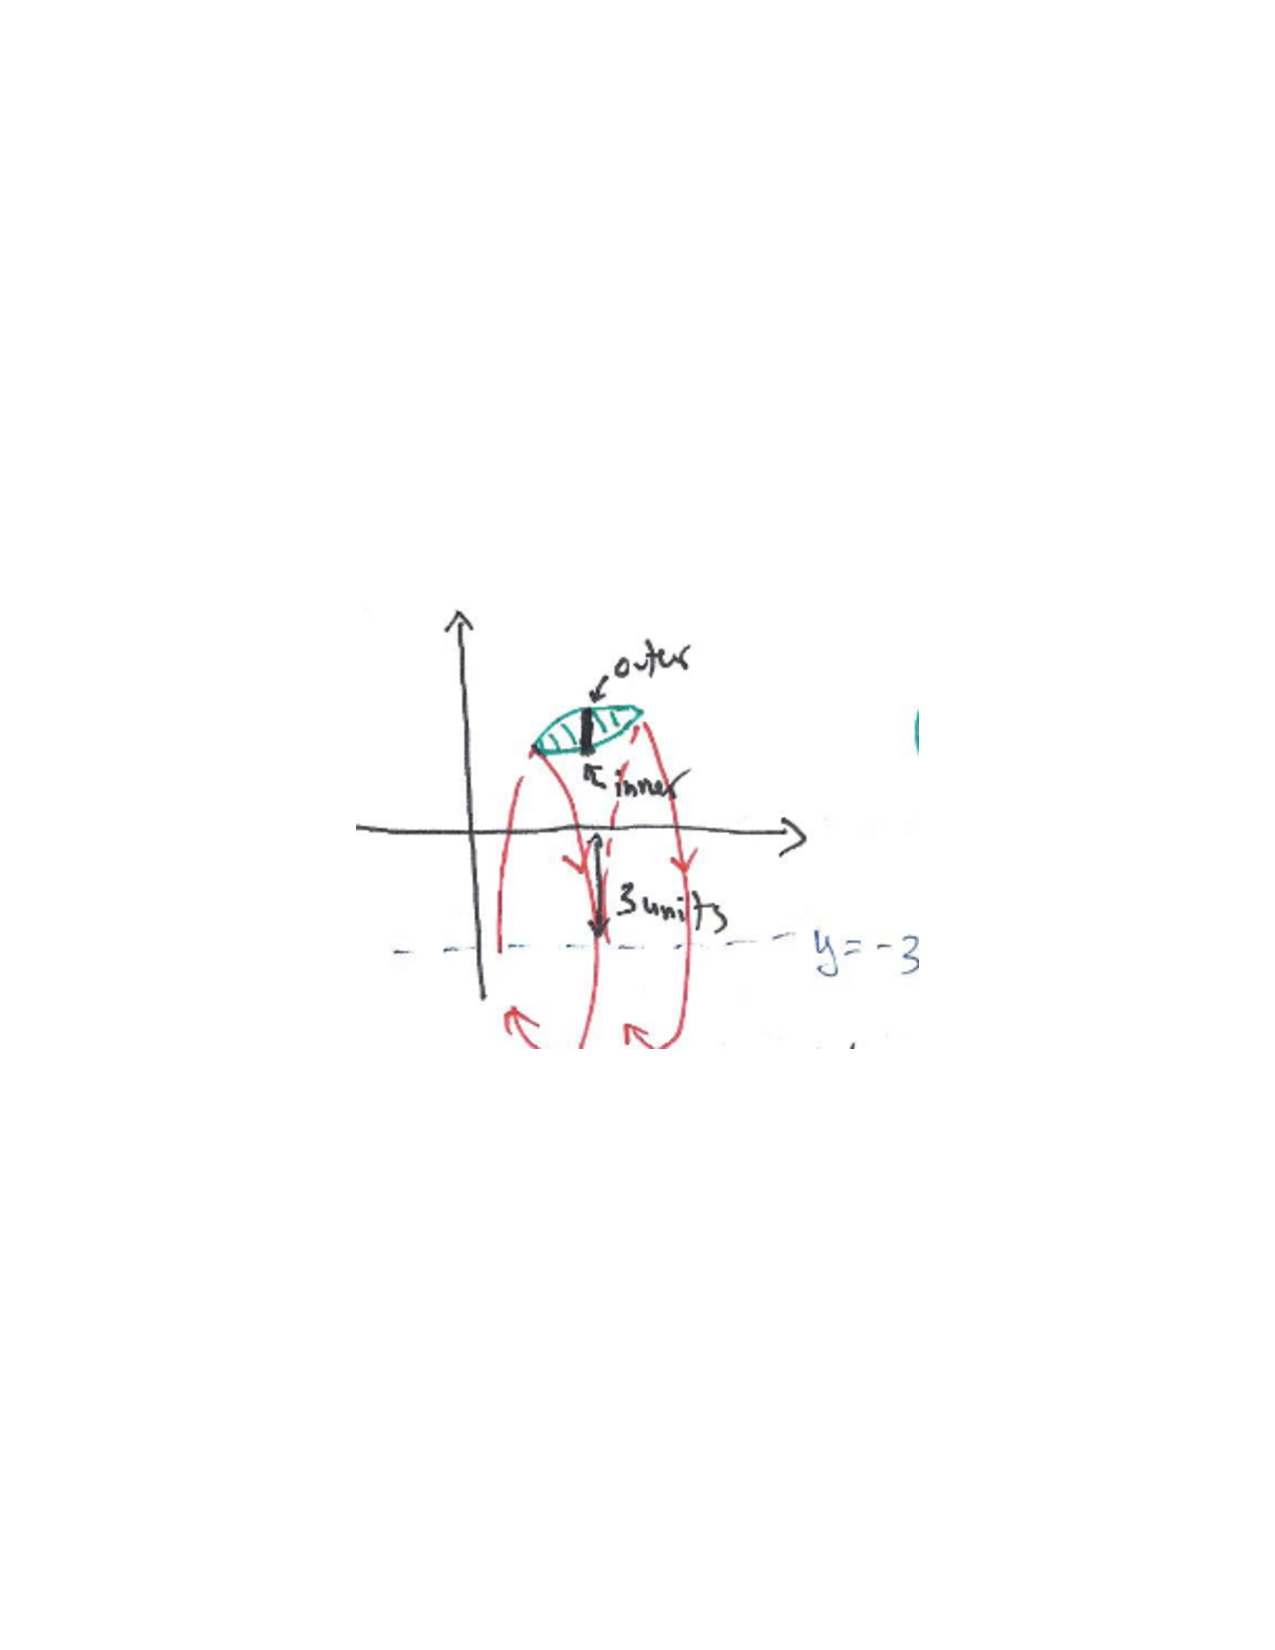
\includegraphics[trim= 240 290 200 280, scale=0.8]{Figure6-3-5.pdf}
		\end{image}
		\end{freeResponse}
		
		
		
		\item  $y=15$
		\begin{freeResponse}
		Now, the line $y=15$ is the $x$-axis shifted up 15 units.  
		This causes a bigger difference than in part (b), since our axis of rotation has moved to the opposite side of the region between the curves.  
		Consulting the picture below, we see that
			\begin{align*}
			r_{out} &= 15 - (x^2-4x+8) = -x^2 + 4x + 7  \\
			r_{in} &= 15 - (-x^2 + 10x - 12) = x^2 - 10x + 27.
			\end{align*}
		Then
			\[
			\text{{\color{red} Volume of region}} = \pi \int_2^5 \left[ (-x^2+4x+7)^2 - (x^2-10x+27)^2 \right] \d x.
			\]
			
		\begin{image}
		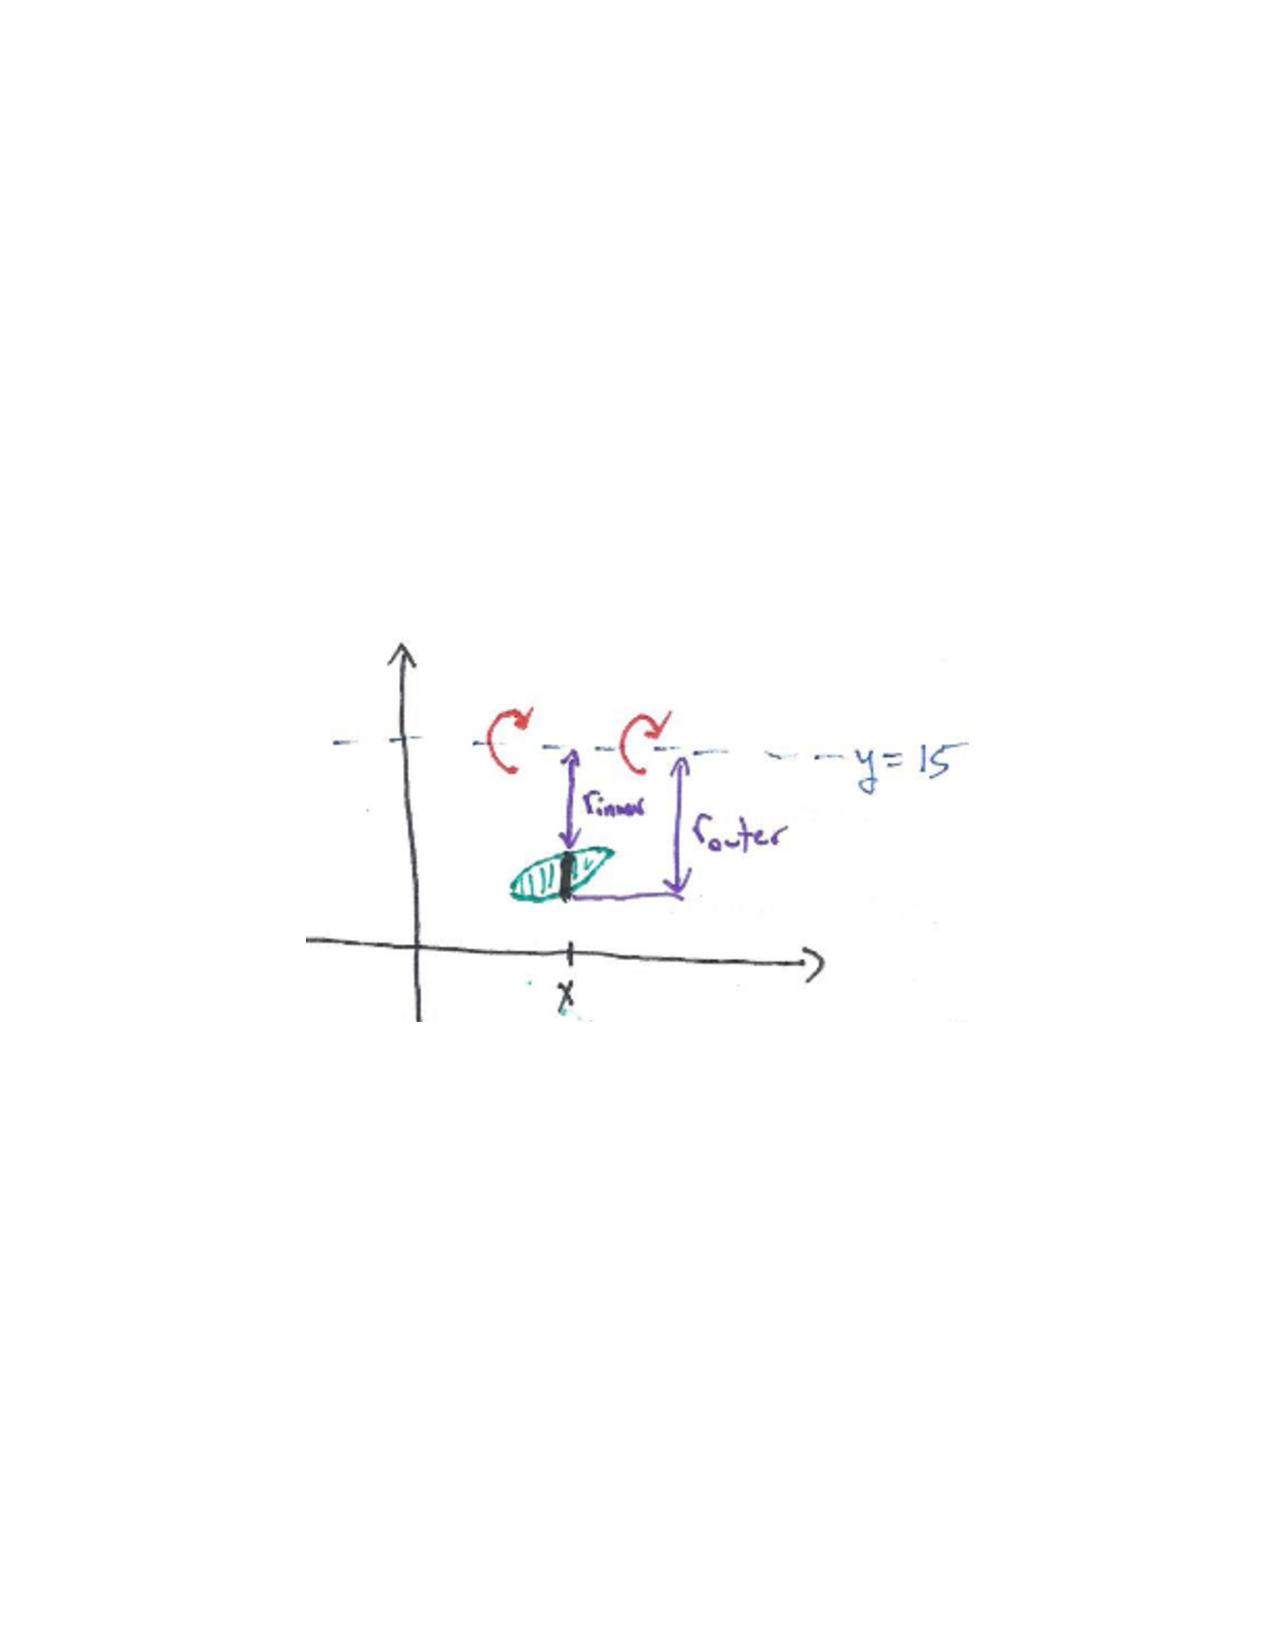
\includegraphics[trim= 240 310 200 310, scale=0.8]{Figure6-3-6.pdf}
		\end{image}
		\end{freeResponse}
		
	\end{enumerate}
		
\end{problem}

\begin{instructorNotes}
Split the parts between the different groups and allow students to present.
\end{instructorNotes}




\begin{problem}
Set up an integral that will compute the volume of the solid generated by revolving the region bounded by the curves $y=x^2-6x+13$ (i.e. $x = 3 \pm \sqrt{y-4}$) and $y=3x-1$ about:

\begin{image}
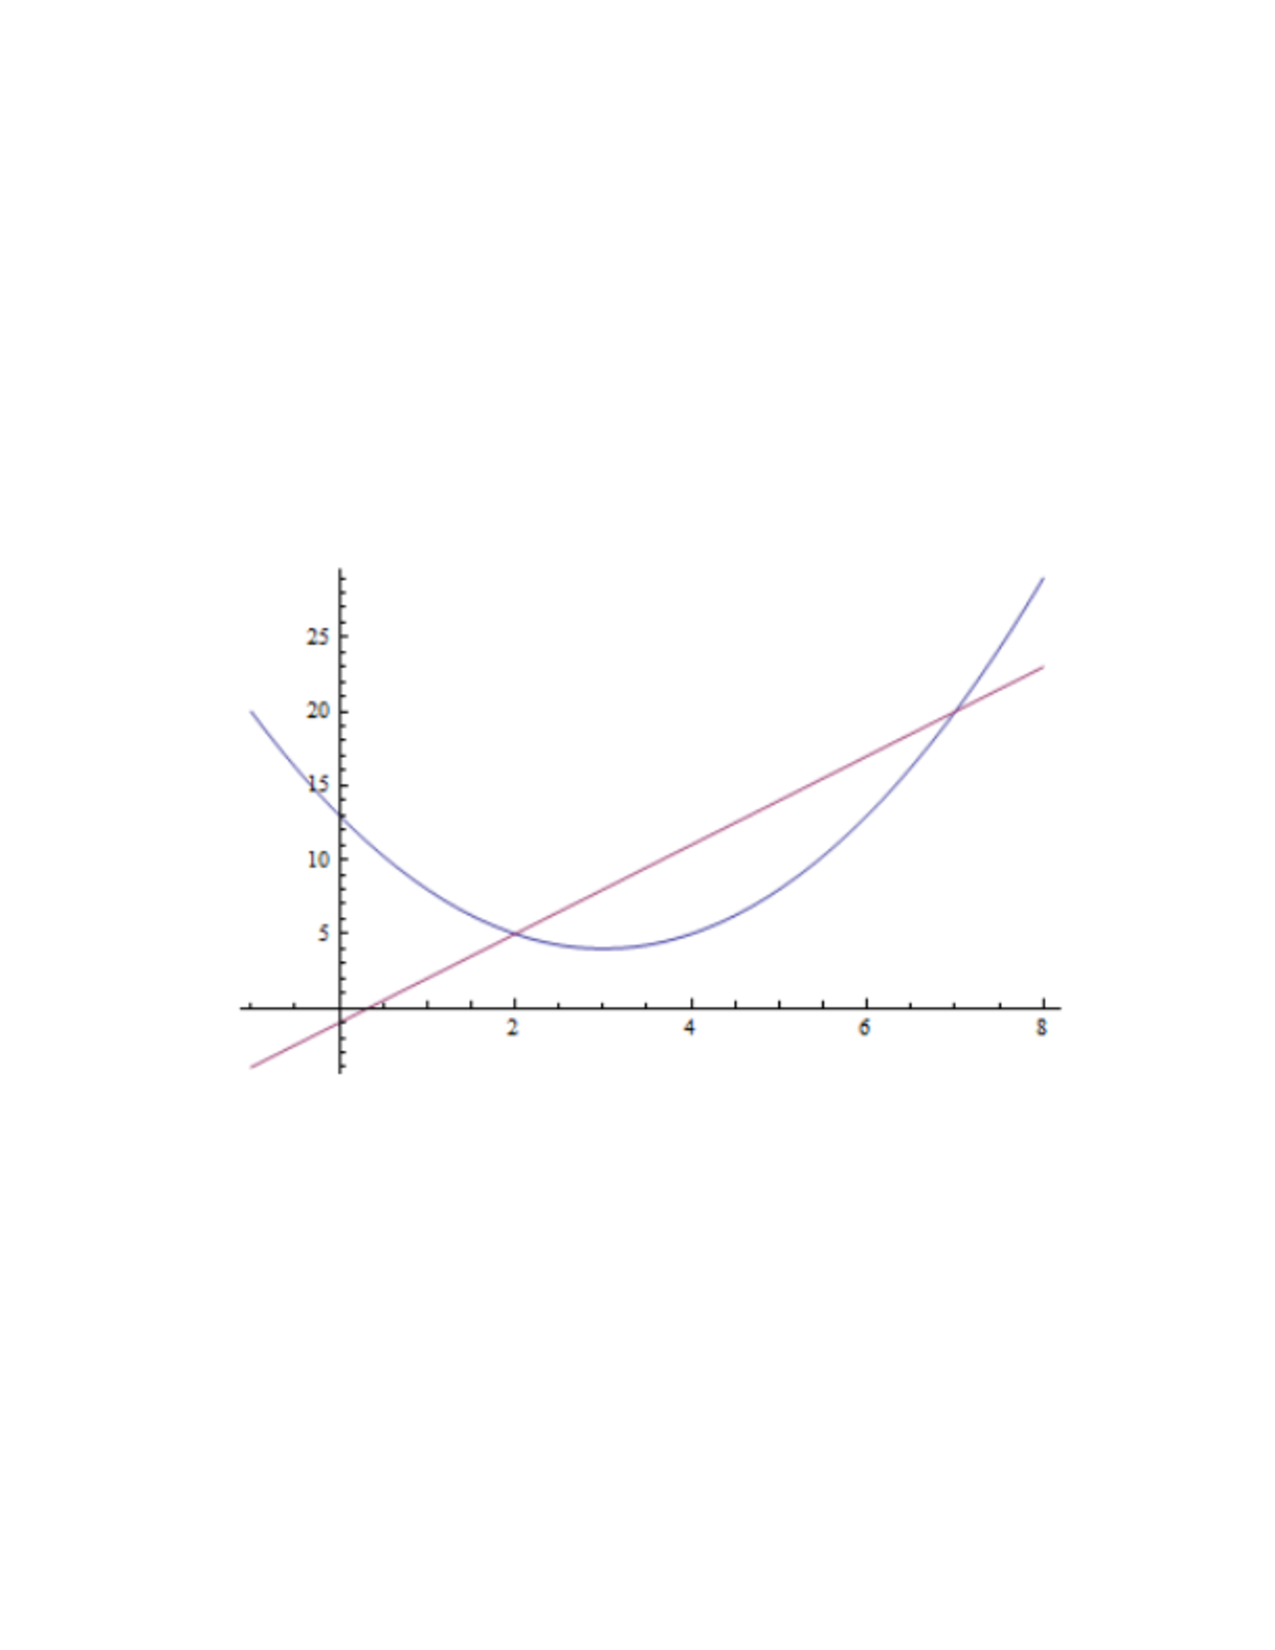
\includegraphics[trim= 170 270 150 280, scale=0.8]{Figure6-4-1.pdf}
\end{image}

Use both the washer method as well as the shell method for each problem.  
Which method would you prefer for each problem?  Why?

	\begin{enumerate}
		\item  the $x$-axis
		\begin{freeResponse}
		First, we need to find the points where the curves intersect
			\begin{align*}
			x^2 - 6x + 13 &= 3x - 1  \\
			x^2 - 9x + 14 &= 0  \\
			(x-2)(x-7) &= 0  \\
			x &= 2, 7  \\
			(2,5&), (7,20).
			\end{align*}
		As we will see later, we also need to locate the vertex of the parabola $x^2 - 6x + 13$.  
		So we complete the square
			\begin{align*}
			y &= x^2 - 6x + 13  \\
			&= (x^2 - 6x \, {\color{red} + \, 9}) + 13 \, {\color{red} - \, 9}  \\
			&= (x-3)^2 + 4.
			\end{align*}
		So the vertex of the parabola is $(3,4)$.  
		
		\begin{image}
		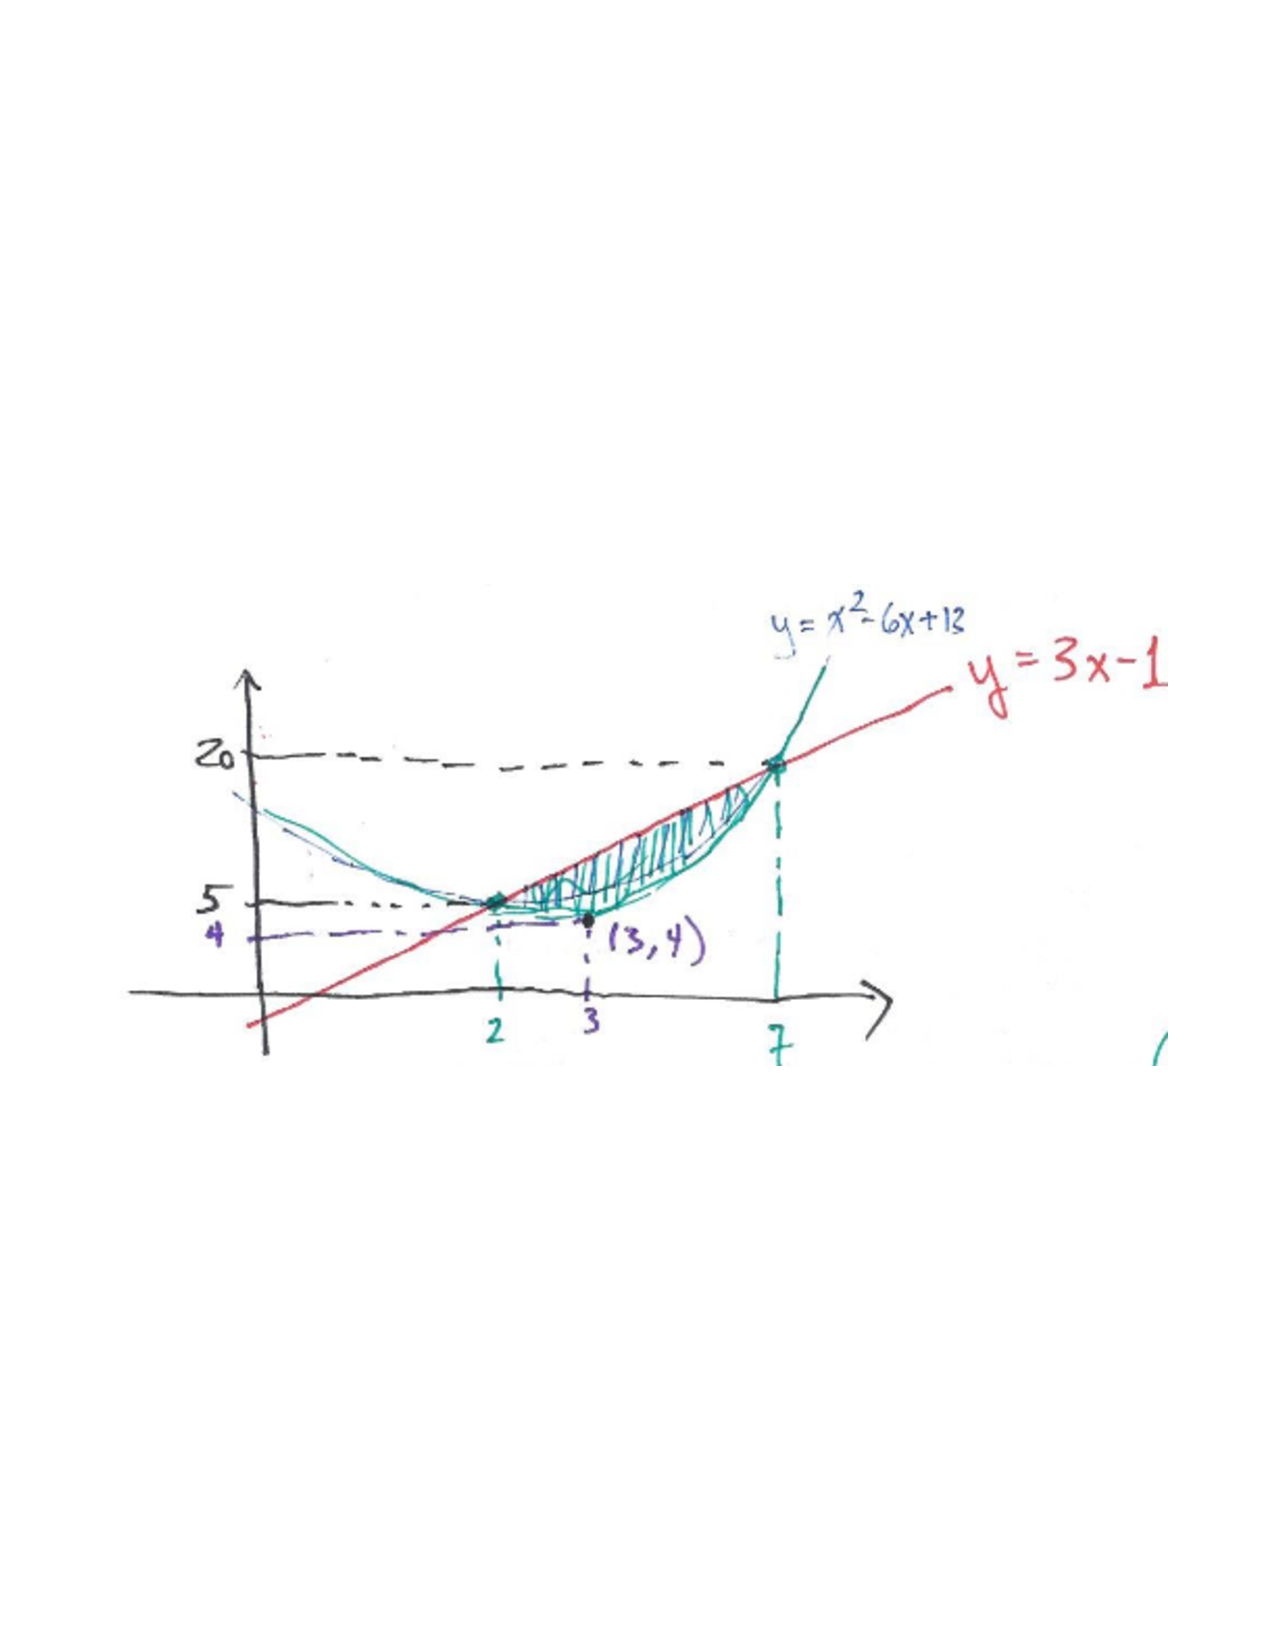
\includegraphics[trim= 170 270 150 280, scale=0.8]{Figure6-4-2.pdf}
		\end{image}

		{\bf Washers: }  For washers, the cross-sections must be \dfn{perpendicular} to the axis of rotation.  
		So here we integrate along the $x$-axis.  
		We have that
			\begin{align*}
			r_{out} &= 3x-1 \\
			r_{in} &= x^2 - 6x +13
			\end{align*}
		and
			\[
			\text{{\color{red} Volume of the region}} = \pi \int_2^7 \left[ (3x-1)^2 - (x^2-6x+13)^2 \right] \d x.
			\]
			
		\begin{image}
		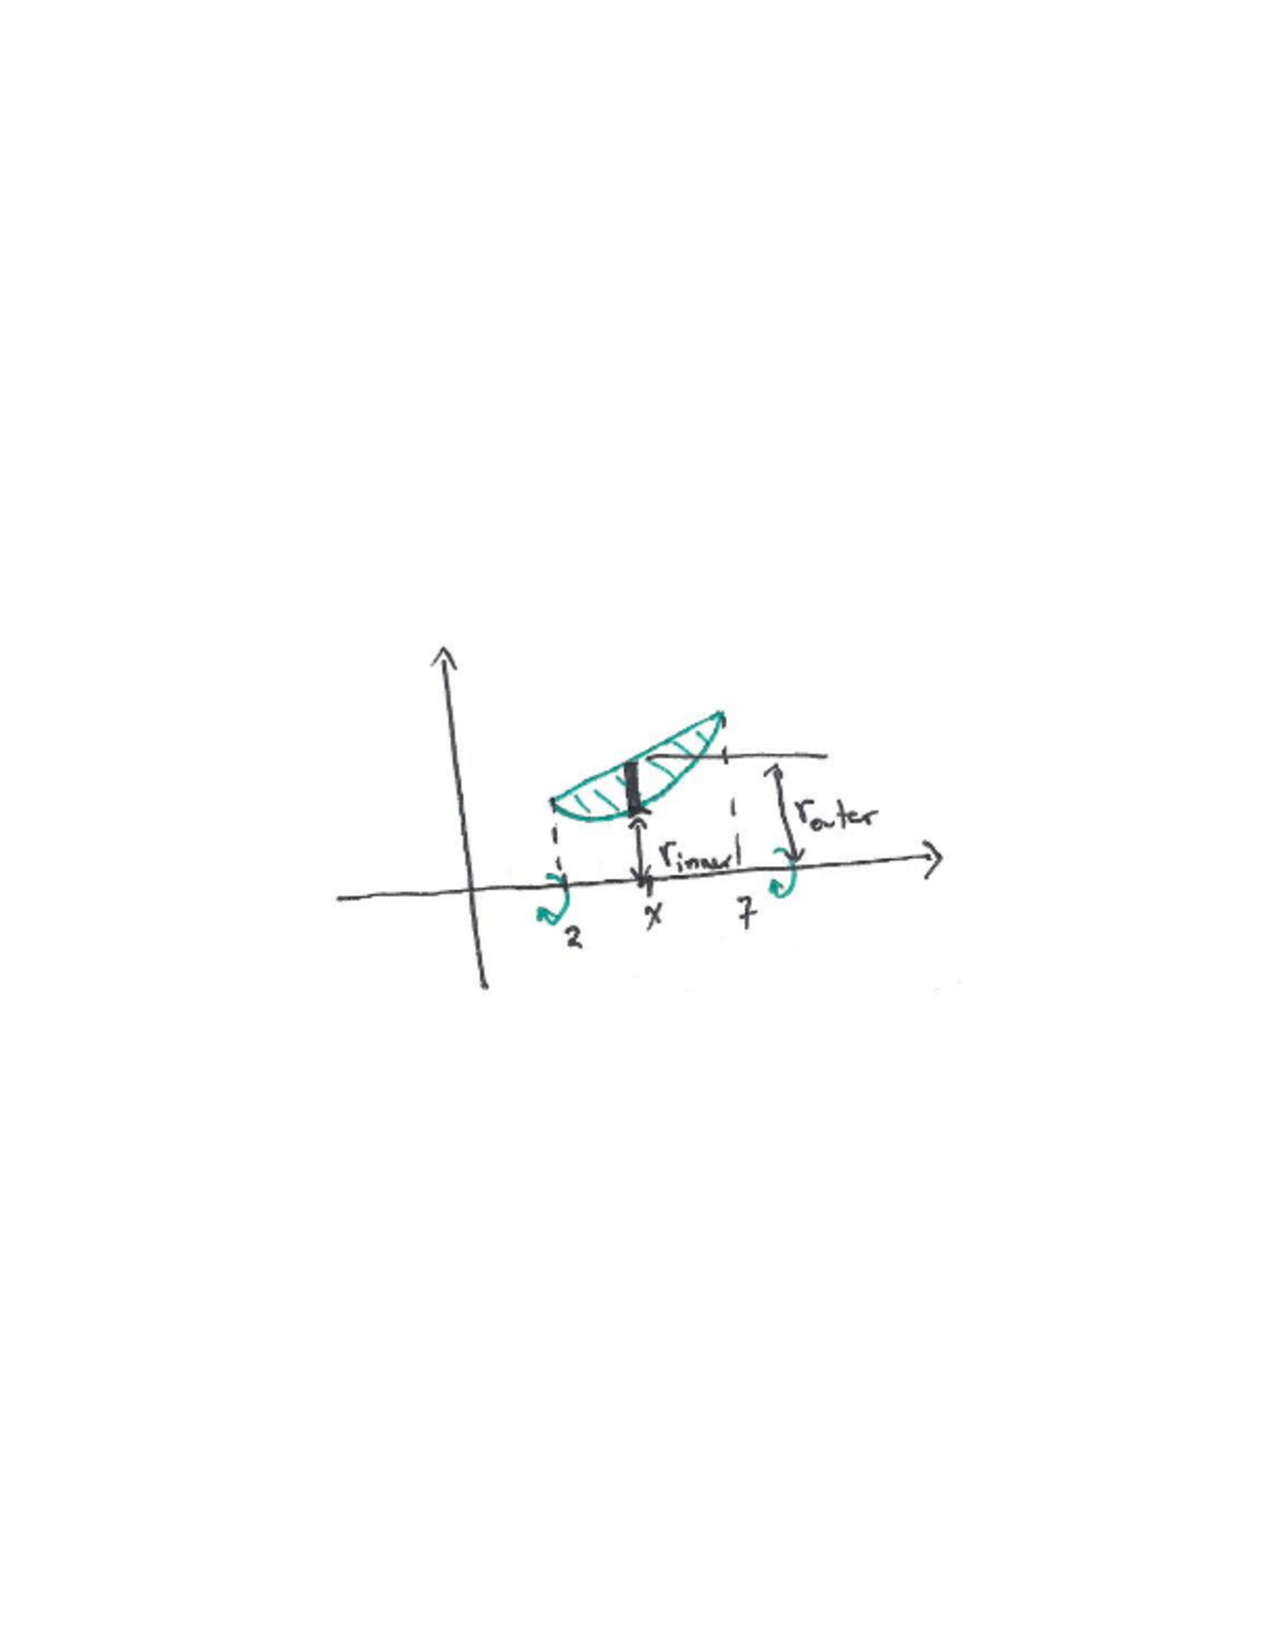
\includegraphics[trim= 200 320 150 310, scale=0.8]{Figure6-4-3.pdf}
		\end{image}
		
		{\bf Shells: }
		For shells, the cross-sections must be \dfn{parallel} to the axis of rotation.  
		So here we integrate along the $y$-axis, $5 \leq y \leq 20$.  
		But we have a problem, namely the ``bottom" of each cross-section changes at $y=5$ due to the shape of the region (see the picture below).
		So we have two different cases:
			\begin{enumerate}
			\item[(1)]  For $4 \leq y \leq 5$
				\begin{align*}
				h &= (3+\sqrt{y-1}) - (3-\sqrt{y-1}) = 2\sqrt{y-1}  \\
				r &= y
				\end{align*}
				
			\item[(2)]  For $5 \leq y \leq 20$
				\begin{align*}
				h &= (3+\sqrt{y-1}) - \left( \frac{1}{3} (y+1) \right)  \\
				r &= y.
				\end{align*}
			\end{enumerate}
		Thus
			\[
			V = \int_4^{20} 2 \pi r h \d y = 2\pi \left[ \int_4^5 y \cdot 2\sqrt{y-1} \d y + \int_5^{20} y \left( (3 + \sqrt{y+1}) - \frac{1}{3}(y+1) \right) \d y \right]
			\]
		
		\begin{image}
		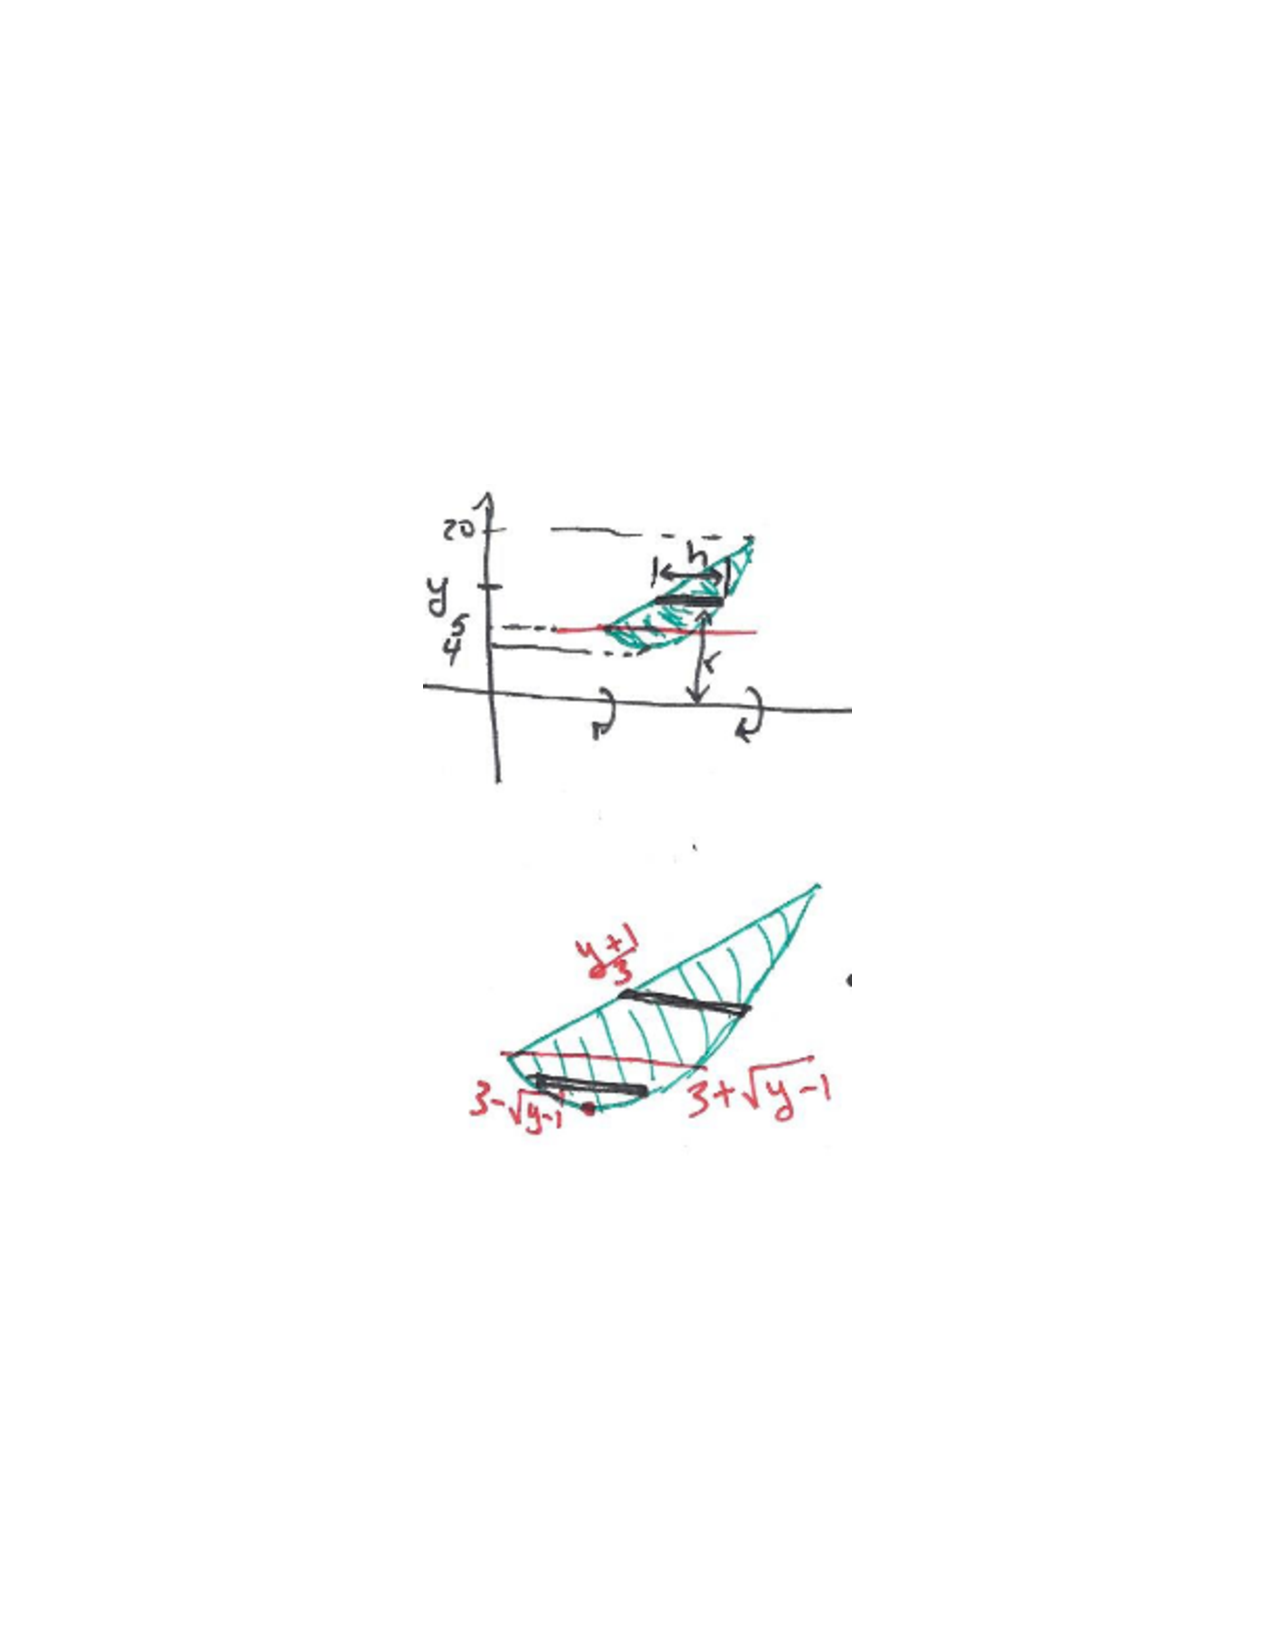
\includegraphics[trim= 200 240 150 240, scale=1]{Figure6-4-4.pdf}
		\end{image}
		
		It is pretty clear in this problem that the washer's method was easier than the shell's method.
		\end{freeResponse}
		
		
		
		
			

		
		
		
		
	\end{enumerate}
	
\end{problem}

\begin{instructorNotes}
Split the two methods between groups.  As a class, discuss which method was better to use in this circumstance.
\end{instructorNotes}



















	
	
	
	
	
	
	
	
	

	










								
				
				
	














\end{document} 


















